\begin{flushright} {\tiny {\color{gray} python\_codes/fieldstone\_115/text.tex}} \end{flushright}

\lstinputlisting[language=bash,basicstyle=\small]{python_codes/fieldstone_115/keywords.ascii}

\begin{center}
\fbox{\textbf{\huge \color{teal} P}}
Codes at \url{https://github.com/cedrict/fieldstone/tree/master/python_codes/fieldstone_115}
\end{center}

\par\noindent\rule{\textwidth}{0.4pt}

%%%%%%%%%%%%%%%%%%%%%%%%%%%%%%%%%%%%%%%%%%%%%%%%%%%%%%%%%%%%%%%%%%%%%%%%%%%%%%%%%%%%%%%%%%%%%%



When it comes to the stabilisation of the $Q_1\times P_0$ elements, 
we have seen in Section~\ref{ss:pairq1p0stab} that mulitple types co-exist
and that a tuning parameter $\epsilon$ plays a role. 
Despite the published literature on the topic, the following questions remain:

- how to deal with vicosity contrasts ? 

- which stab is best for real life geodynamics ? 

- how to deal with not square mesh ?

- how to choose the $\epsilon$ value ?

- look at buoyancy driven flows. lith pressure!

- I have implemented penalty, global, local and macro-element. what about the other methods, eg bodg06 ?

- concretely how would PCG converge?

The code is based on \stone 14.

Velocity divergence is measured at the center of the element.

note that in case of penalty, $\epsilon$ should be $\sim 10^6$ larger than viscosity.

%====================================================================================
\subsection*{Donea \& Huerta manufactured solution}


\begin{center}
\includegraphics[width=5cm]{python_codes/fieldstone_115/results/dh/nostab/matrix}
\includegraphics[width=5cm]{python_codes/fieldstone_115/results/dh/penalty/matrix}
\includegraphics[width=5cm]{python_codes/fieldstone_115/results/dh/global/matrix}\\
\includegraphics[width=5cm]{python_codes/fieldstone_115/results/dh/local/matrix}
\includegraphics[width=5cm]{python_codes/fieldstone_115/results/dh/macro/matrix}\\
{\captionfont 32x32. From left to right: parsity pattern of the FEM matric for 
no stabilisation, penalty, global, local, macro-elt.}
\end{center}

We find that all three stabilisation $\C$ matrices are enough to suppress the chequerboard mode:
\begin{center}
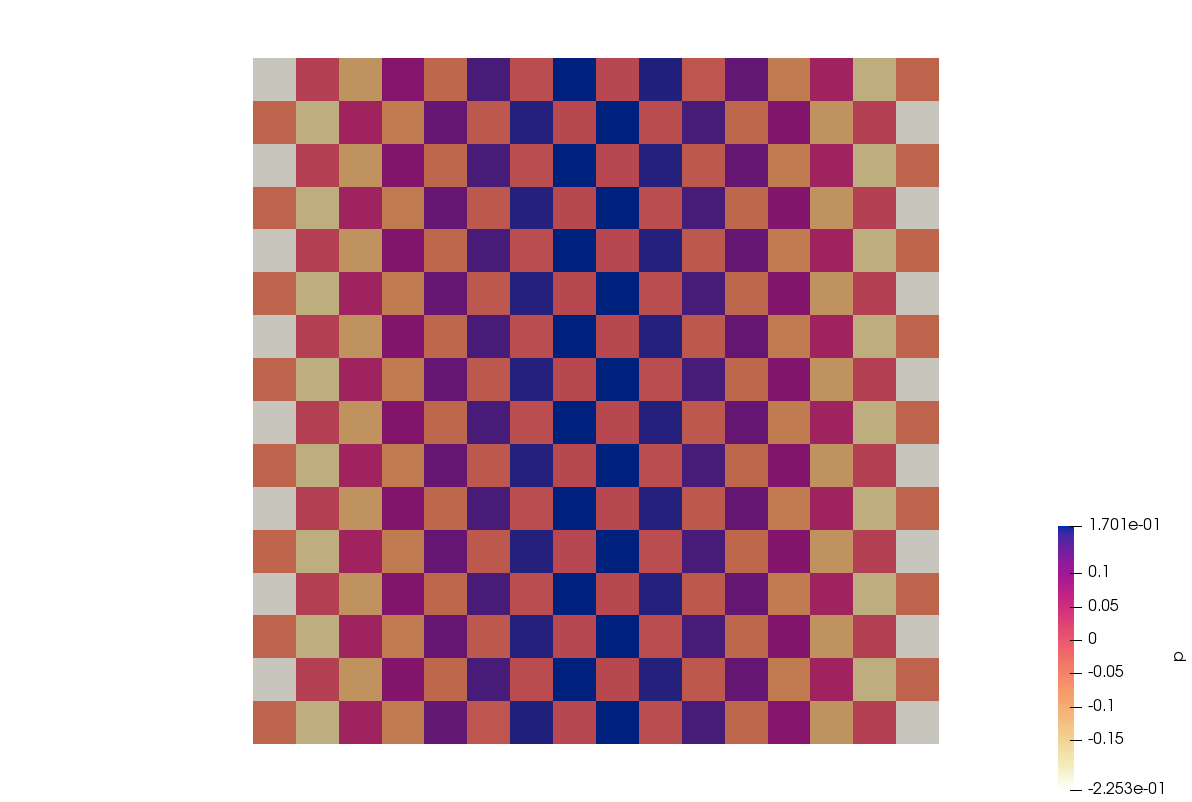
\includegraphics[width=3.4cm]{python_codes/fieldstone_115/results/dh/p0}
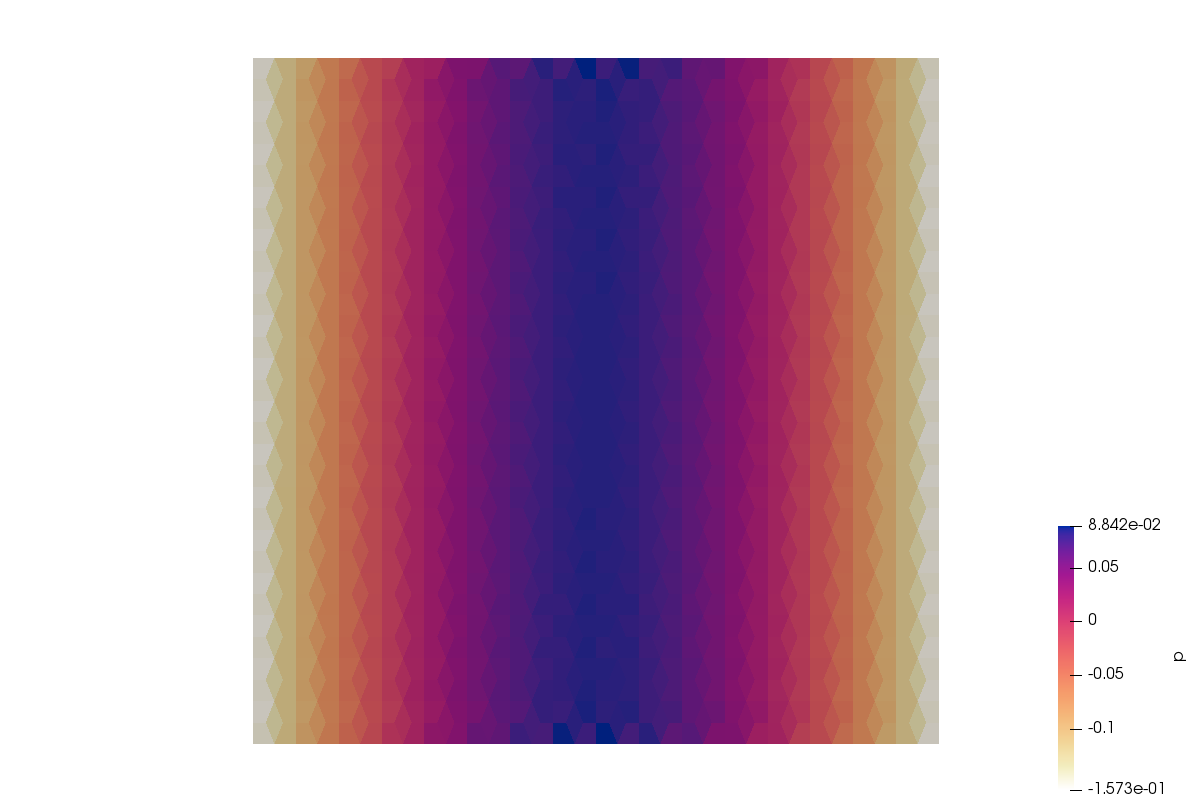
\includegraphics[width=3.4cm]{python_codes/fieldstone_115/results/dh/p1}
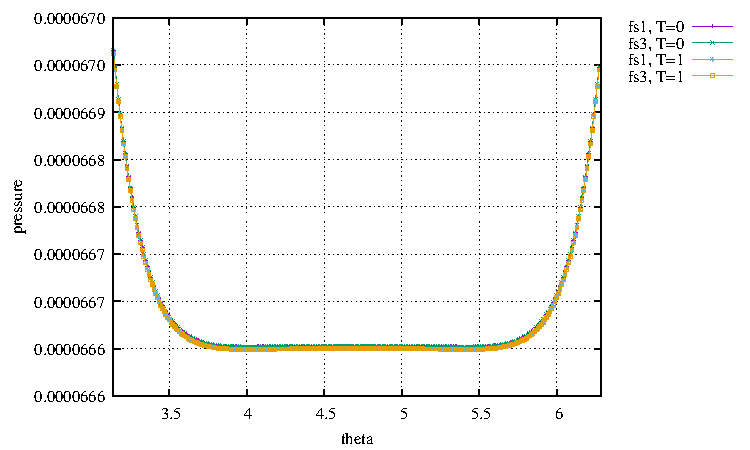
\includegraphics[width=3.4cm]{python_codes/fieldstone_115/results/dh/p2}
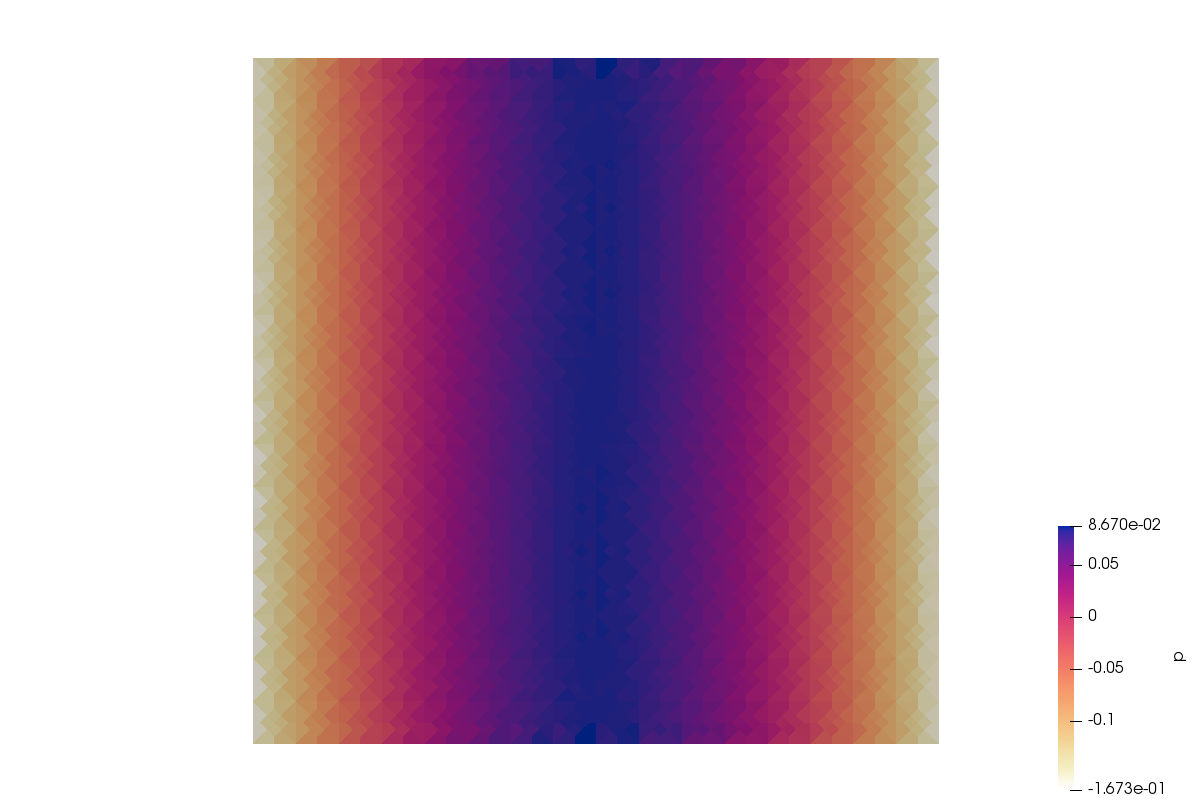
\includegraphics[width=3.4cm]{python_codes/fieldstone_115/results/dh/p3}
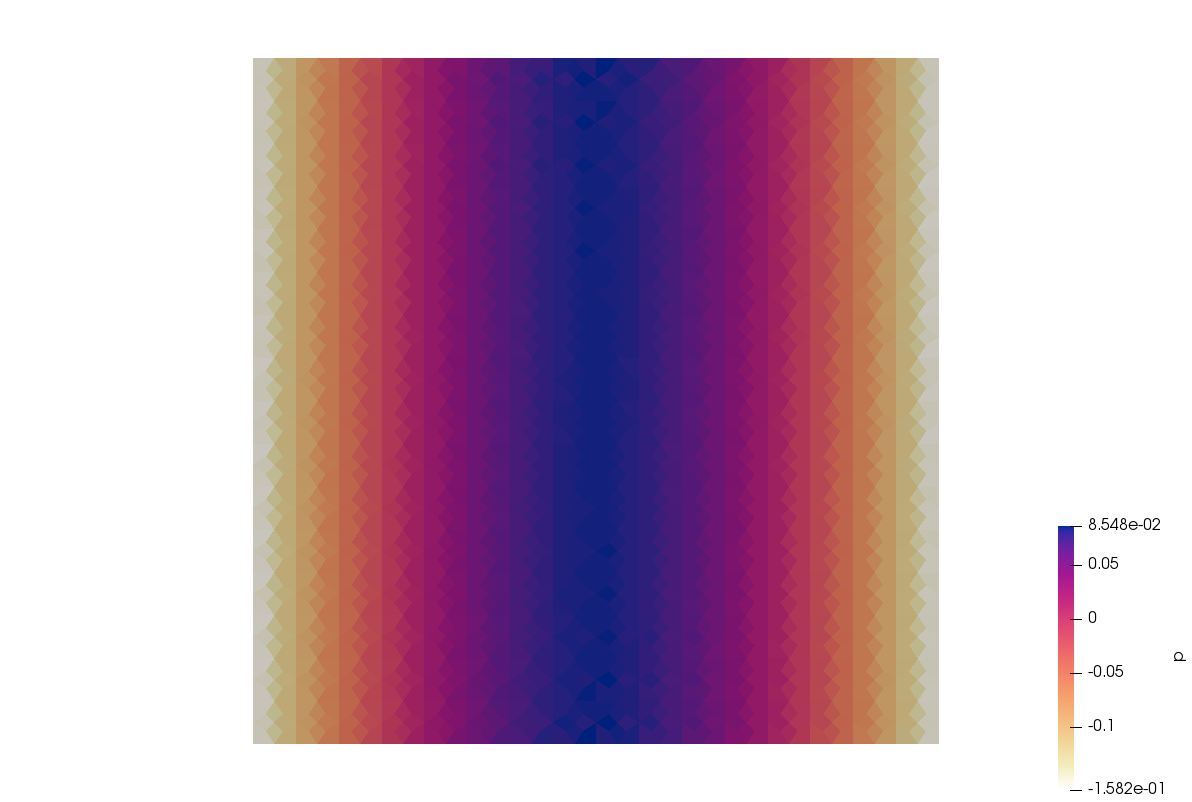
\includegraphics[width=3.4cm]{python_codes/fieldstone_115/results/dh/p4}\\
{\captionfont resolution $32\times 32$. From left to right: no stabilisation, penalty, 
global, local, macro-elt. $\epsilon=10^{-1}$}
\end{center}

We can now explore the influence of the stabilisation parameter $\epsilon$. Obviously, 
if too low it won't have any effect as the $\C$ matrix then tends to zero. If too high,
then we expect it to perturb the solution too much. 
The pressure field is shown in the following figure for various values of $\epsilon$, 


\begin{center}
\includegraphics[width=3.4cm]{python_codes/fieldstone_115/results/dh/pressure_nostab.pdf}
\includegraphics[width=3.4cm]{python_codes/fieldstone_115/results/dh/pressure_penalty.pdf}
\includegraphics[width=3.4cm]{python_codes/fieldstone_115/results/dh/pressure_global.pdf}
\includegraphics[width=3.4cm]{python_codes/fieldstone_115/results/dh/pressure_local.pdf}
\includegraphics[width=3.4cm]{python_codes/fieldstone_115/results/dh/pressure_macro.pdf}\\
\includegraphics[width=3.4cm]{python_codes/fieldstone_115/results/dh/pressure_nostab_error.pdf}
\includegraphics[width=3.4cm]{python_codes/fieldstone_115/results/dh/pressure_penalty_error.pdf}
\includegraphics[width=3.4cm]{python_codes/fieldstone_115/results/dh/pressure_global_error.pdf}
\includegraphics[width=3.4cm]{python_codes/fieldstone_115/results/dh/pressure_local_error.pdf}
\includegraphics[width=3.4cm]{python_codes/fieldstone_115/results/dh/pressure_macro_error.pdf}\\
{\captionfont 32x32. pressure profile.} 
\end{center}

Let us now turn to the velocity and pressure error convergence rates: 
\begin{center}
\includegraphics[width=4.21cm]{python_codes/fieldstone_115/results/dh/errorsV_penalty.pdf}
\includegraphics[width=4.21cm]{python_codes/fieldstone_115/results/dh/errorsV_global.pdf}
\includegraphics[width=4.21cm]{python_codes/fieldstone_115/results/dh/errorsV_local.pdf}
\includegraphics[width=4.21cm]{python_codes/fieldstone_115/results/dh/errorsV_macro.pdf}\\
\includegraphics[width=4.21cm]{python_codes/fieldstone_115/results/dh/errorsP_penalty.pdf}
\includegraphics[width=4.21cm]{python_codes/fieldstone_115/results/dh/errorsP_global.pdf}
\includegraphics[width=4.21cm]{python_codes/fieldstone_115/results/dh/errorsP_local.pdf}
\includegraphics[width=4.21cm]{python_codes/fieldstone_115/results/dh/errorsP_macro.pdf}\\
\includegraphics[width=4.21cm]{python_codes/fieldstone_115/results/dh/divv_penalty.pdf}
\includegraphics[width=4.21cm]{python_codes/fieldstone_115/results/dh/divv_global.pdf}
\includegraphics[width=4.21cm]{python_codes/fieldstone_115/results/dh/divv_local.pdf}
\includegraphics[width=4.21cm]{python_codes/fieldstone_115/results/dh/divv_macro.pdf}\\
{\captionfont Velocity and pressure errors as a function of the element size for meshes 6x6 to 144x144}
\end{center}
We find that the error convergence rate for velocity is always quadratic as expected, 
while the error convergence for pressure becomes monotonous and linear as expected too.

It also appears that the macro-element technique is the least sensitive to the value of $\epsilon$, 
although it is rather surprising that even very low values of $\epsilon$ manage to stabilise the 
system so well. could it be because this benchmark is very smooth? 
\begin{center}
\includegraphics[width=5.7cm]{python_codes/fieldstone_115/results/dh/errorsP_32_eps}
\includegraphics[width=5.7cm]{python_codes/fieldstone_115/results/dh/errorsP_64_eps}
\includegraphics[width=5.7cm]{python_codes/fieldstone_115/results/dh/errorsP_96_eps}\\
{\captionfont Influence of $\epsilon$ parameter on pressure error.}
\end{center}

{\bf Conclusion}: macro-element technique yields best results: lower velocity divergence, 
least sensitive to $\epsilon$ value, block matrix,

I should monitor the condition number of the matrix...

\newpage
%====================================================================================
\subsection*{The aquarium}

The domain is still a unit square. Boundary conditions are no slip on all sides. 
Density and viscosity are set to 1. Gravity is vertical with $\vec{g}=-\vec{e}_y$.
The analytical velocity is obviously $\vec\upnu=\vec{0}$ and the analytical pressure
is $p(x,y)=0.5-y$ (which fulfils $\int_\Omega p dV=0$).

Because the analytical velocity field is a constant, it can be represented exactly 
by bi-linear functions so we expect the velocity error to be at machine precision
independently of the resolution. However, because of the presence of the stabilisation
term, we find in the penalty case that it is proportional to $\epsilon$ and 
in the global and local cases that it converges quadratically.

The analytical pressure field, on the other hand is a linear polynomial which cannot 
be represented exactly by a set of discontinuous $C^0$ functions. We then expect and 
indeed recover a linear convergence.


\begin{center}
\includegraphics[width=4.21cm]{python_codes/fieldstone_115/results/aquarium/errorsV_penalty.pdf}
\includegraphics[width=4.21cm]{python_codes/fieldstone_115/results/aquarium/errorsV_global.pdf}
\includegraphics[width=4.21cm]{python_codes/fieldstone_115/results/aquarium/errorsV_local.pdf}
\includegraphics[width=4.21cm]{python_codes/fieldstone_115/results/aquarium/errorsV_macro.pdf}\\
\includegraphics[width=4.21cm]{python_codes/fieldstone_115/results/aquarium/errorsP_penalty.pdf}
\includegraphics[width=4.21cm]{python_codes/fieldstone_115/results/aquarium/errorsP_global.pdf}
\includegraphics[width=4.21cm]{python_codes/fieldstone_115/results/aquarium/errorsP_local.pdf}
\includegraphics[width=4.21cm]{python_codes/fieldstone_115/results/aquarium/errorsP_macro.pdf}\\
\includegraphics[width=4.21cm]{python_codes/fieldstone_115/results/aquarium/divv_penalty.pdf}
\includegraphics[width=4.21cm]{python_codes/fieldstone_115/results/aquarium/divv_global.pdf}
\includegraphics[width=4.21cm]{python_codes/fieldstone_115/results/aquarium/divv_local.pdf}
\includegraphics[width=4.21cm]{python_codes/fieldstone_115/results/aquarium/divv_macro.pdf}\\
{\captionfont Velocity and pressure errors as a function of the element size for meshes 6x6 to 144x144}
\end{center}


\begin{center}
\includegraphics[width=5.7cm]{python_codes/fieldstone_115/results/aquarium/errorsP_32_eps}
\includegraphics[width=5.7cm]{python_codes/fieldstone_115/results/aquarium/errorsP_64_eps}
\includegraphics[width=5.7cm]{python_codes/fieldstone_115/results/aquarium/errorsP_96_eps}\\
{\captionfont Influence of $\epsilon$ parameter on pressure error.}
\end{center}


\newpage
%====================================================================================
\subsection*{Lid driven cavity}

This is not a benchmark but a simple setup which is not very physical. The most right and left
points of the lid have zero velocity ('non-leaky cavity').

We find that in the absence of stabilisation the pressure chequerboard mode is 
very strong:
\begin{center}
\includegraphics[width=5.7cm]{python_codes/fieldstone_115/results/ldc/nostab/vel}
\includegraphics[width=5.7cm]{python_codes/fieldstone_115/results/ldc/nostab/p}
\includegraphics[width=5.7cm]{python_codes/fieldstone_115/results/ldc/psurf_nostab.pdf}\\
{\captionfont No stabilisation: velocity and pressure at 32x32. Right: 
pressure at the top at various resolutions.}
\end{center}

\begin{center}
\includegraphics[width=5.7cm]{python_codes/fieldstone_115/results/ldc/psurf_penalty.pdf}
\includegraphics[width=5.7cm]{python_codes/fieldstone_115/results/ldc/psurf_global.pdf}\\
\includegraphics[width=5.7cm]{python_codes/fieldstone_115/results/ldc/psurf_local.pdf}
\includegraphics[width=5.7cm]{python_codes/fieldstone_115/results/ldc/psurf_macro.pdf}\\
{\captionfont Pressure at the top at $128\times 128$ resolution.}
\end{center}

\begin{center}
\includegraphics[width=4cm]{python_codes/fieldstone_115/results/ldc/vrms_penalty.pdf}
\includegraphics[width=4cm]{python_codes/fieldstone_115/results/ldc/vrms_global.pdf}
\includegraphics[width=4cm]{python_codes/fieldstone_115/results/ldc/vrms_local.pdf}
\includegraphics[width=4cm]{python_codes/fieldstone_115/results/ldc/vrms_macro.pdf}\\
\includegraphics[width=4cm]{python_codes/fieldstone_115/results/ldc/prms_penalty.pdf}
\includegraphics[width=4cm]{python_codes/fieldstone_115/results/ldc/prms_global.pdf}
\includegraphics[width=4cm]{python_codes/fieldstone_115/results/ldc/prms_local.pdf}
\includegraphics[width=4cm]{python_codes/fieldstone_115/results/ldc/prms_macro.pdf}\\
\includegraphics[width=4cm]{python_codes/fieldstone_115/results/ldc/divv_penalty.pdf}
\includegraphics[width=4cm]{python_codes/fieldstone_115/results/ldc/divv_global.pdf}
\includegraphics[width=4cm]{python_codes/fieldstone_115/results/ldc/divv_local.pdf}
\includegraphics[width=4cm]{python_codes/fieldstone_115/results/ldc/divv_macro.pdf}\\
{\captionfont Left to right: penalty, global, local, macro-element}
\end{center}

\newpage
%==============================================================================
\subsection*{Manufactured solution of \textcite{buha06}}

See section~\ref{ss:mms_buha06}.
The velocity and pressure fields are given in the unit square by
\begin{eqnarray}
u(x,y) &=& 20xy^3 \nn\\
v(x,y) &=& 5x^4-5y^4 \nn\\
p(x,y) &=& 60x^2y -20y^3 -5
\end{eqnarray}


\begin{center}
\includegraphics[width=4cm]{python_codes/fieldstone_115/results/buha06/errorsV_penalty.pdf}
\includegraphics[width=4cm]{python_codes/fieldstone_115/results/buha06/errorsV_global.pdf}
\includegraphics[width=4cm]{python_codes/fieldstone_115/results/buha06/errorsV_local.pdf}
\includegraphics[width=4cm]{python_codes/fieldstone_115/results/buha06/errorsV_macro.pdf}\\
\includegraphics[width=4cm]{python_codes/fieldstone_115/results/buha06/errorsP_penalty.pdf}
\includegraphics[width=4cm]{python_codes/fieldstone_115/results/buha06/errorsP_global.pdf}
\includegraphics[width=4cm]{python_codes/fieldstone_115/results/buha06/errorsP_local.pdf}
\includegraphics[width=4cm]{python_codes/fieldstone_115/results/buha06/errorsP_macro.pdf}\\
\includegraphics[width=4cm]{python_codes/fieldstone_115/results/buha06/divv_penalty.pdf}
\includegraphics[width=4cm]{python_codes/fieldstone_115/results/buha06/divv_global.pdf}
\includegraphics[width=4cm]{python_codes/fieldstone_115/results/buha06/divv_local.pdf}
\includegraphics[width=4cm]{python_codes/fieldstone_115/results/buha06/divv_macro.pdf}\\
{\captionfont Velocity and pressure errors as a function of the element size for meshes 6x6 to 144x144.
Left to right: penalty, global, local, macro-element}
\end{center}



\begin{center}
\includegraphics[width=3.2cm]{python_codes/fieldstone_115/results/buha06/p0}
\includegraphics[width=3.2cm]{python_codes/fieldstone_115/results/buha06/p1}
\includegraphics[width=3.2cm]{python_codes/fieldstone_115/results/buha06/p2}
\includegraphics[width=3.2cm]{python_codes/fieldstone_115/results/buha06/p3}
\includegraphics[width=3.2cm]{python_codes/fieldstone_115/results/buha06/p4}\\
\includegraphics[width=3.2cm]{python_codes/fieldstone_115/results/buha06/divv0}
\includegraphics[width=3.2cm]{python_codes/fieldstone_115/results/buha06/divv1}
\includegraphics[width=3.2cm]{python_codes/fieldstone_115/results/buha06/divv2}
\includegraphics[width=3.2cm]{python_codes/fieldstone_115/results/buha06/divv3}
\includegraphics[width=3.2cm]{python_codes/fieldstone_115/results/buha06/divv4}\\
{\captionfont 64x64, epsi=0.1. Left to right: no stab, penalty, global, local, macro-elt.
Top row is pressure, bottom row is elemental velocity divergence.}
\end{center}



\begin{center}
\includegraphics[width=5.7cm]{python_codes/fieldstone_115/results/buha06/errorsP_32_eps}
\includegraphics[width=5.7cm]{python_codes/fieldstone_115/results/buha06/errorsP_64_eps}
\includegraphics[width=5.7cm]{python_codes/fieldstone_115/results/buha06/errorsP_96_eps}\\
{\captionfont Influence of $\epsilon$ parameter on pressure error for global, local, macro-elt}
\end{center}
